\documentclass[tikz]{standalone}
\usepackage{pgfplots}
\pgfplotsset{compat=1.15}
\usepackage{mathrsfs}
\usetikzlibrary{arrows,calc}
\usepackage{tkz-euclide}
\pagestyle{empty}
\usepackage{fp}

\definecolor{AngleClr}{rgb}{0,0.39215686274509803,0}
\definecolor{ShapeClr}{rgb}{0.6,0.2,0}

\definecolor{BlueClr}{RGB}{5,81,163}

\begin{document}

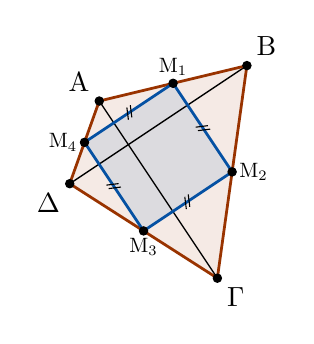
\begin{tikzpicture}[scale=.75]
\tkzSetUpLine[line width=1pt,color=black]
\tkzSetUpPoint[fill=black]

\tkzDefPoints{-0.5/0.4/A,1.5/-2.6/C,-1/-1/D,2/1/B}

% Find the intersection of the diagonals.
\tkzInterLL(B,D)(A,C) \tkzGetPoint{I}

% Find the four midpoints.
\tkzDefMidPoint(A,B) \tkzGetPoint{M1}
\tkzDefMidPoint(B,C) \tkzGetPoint{M2}
\tkzDefMidPoint(C,D) \tkzGetPoint{M3}
\tkzDefMidPoint(D,A) \tkzGetPoint{M4}

\tkzFillPolygon[fill=ShapeClr,fill opacity=0.1,inner sep=1cm](A,B,C,D)
\tkzFillPolygon[fill=BlueClr,fill opacity=0.1,inner sep=1cm](M1,M2,M3,M4)

% Draw diagonals.
\tkzDrawSegment[line width=0.5pt,color=black](A,C)
\tkzDrawSegment[line width=0.5pt,color=black](B,D)

\tkzDrawPolygon[color=ShapeClr](A,B,C,D)
\tkzDrawPolygon[color=BlueClr](M1,M2,M3,M4)
\tkzDrawPoints[size=3](A,B,C,D,M1,M2,M3,M4)

\tkzLabelPoint[above left](A){$\rm A$}
\tkzLabelPoint[above right](B){$\rm B$}
\tkzLabelPoint[below right](C){$\rm \Gamma$}
\tkzLabelPoint[below left](D){$\rm \Delta$}

\tkzLabelPoint[scale=0.75,above](M1){$\rm M_1$}
\tkzLabelPoint[scale=0.75,right](M2){$\rm M_2$}
\tkzLabelPoint[scale=0.75,below](M3){$\rm M_3$}
\tkzLabelPoint[scale=0.75,left](M4){$\rm M_4$}

\tkzMarkSegments[mark=s||,size=2](M1,M2 M2,M3 M3,M4 M4,M1)

\end{tikzpicture}

\end{document}
